% GPU-Accelerated CF-LIBS — Conference Talk (20 min)
% Beamer presentation for JQSRT paper
\documentclass[aspectratio=169,12pt]{beamer}

% --- Theme and colors ---
\usetheme{metropolis}
\usepackage{appendixnumberbeamer}

% Colorblind-safe palette (same as paper)
\definecolor{cbBlue}{HTML}{0072B2}
\definecolor{cbOrange}{HTML}{D55E00}
\definecolor{cbGreen}{HTML}{009E73}
\definecolor{cbYellow}{HTML}{F0E442}
\definecolor{cbPurple}{HTML}{CC79A7}

\setbeamercolor{frametitle}{bg=cbBlue,fg=white}
\setbeamercolor{progress bar}{fg=cbOrange}
\setbeamercolor{alerted text}{fg=cbOrange}

% --- Packages ---
\usepackage{amsmath,amssymb}
\usepackage{graphicx}
\usepackage{booktabs}
\usepackage{siunitx}
\usepackage{bm}
\usepackage{tikz}
\usepackage{multicol}

\sisetup{
  separate-uncertainty = true,
  multi-part-units = single,
}

% --- Metadata ---
\title{GPU-Accelerated Calibration-Free LIBS via JAX}
\subtitle{76$\times$ Voigt speedup, 13.6$\times$ end-to-end, zero accuracy loss}
\author{Brian Squires}
\institute{[Affiliation]}
\date{2026}

% ============================================================
\begin{document}

% ----------------------------------------------------------
% SLIDE 1: Title
% ----------------------------------------------------------
\begin{frame}[plain]
  \titlepage
\note{
  Good morning. I will present our work on GPU-accelerating the full
  Calibration-Free LIBS computational pipeline using JAX.
  The key message: we achieve up to 76 times speedup on individual kernels
  and 13.6 times end-to-end, with no loss of numerical precision.
  Let me start with why this matters.
}
\end{frame}

% ----------------------------------------------------------
% SLIDE 2: What is LIBS?
% ----------------------------------------------------------
\begin{frame}{What is LIBS?}
  \begin{columns}[T]
    \begin{column}{0.55\textwidth}
      \begin{itemize}
        \item Focused laser pulse ablates sample surface
        \item Transient plasma ($T \sim 0.6$--$1.5$ eV, $n_e \sim 10^{15}$--$10^{17}$ cm$^{-3}$)
        \item Optical emission encodes elemental composition
        \item Applications: geology, industry, cultural heritage, \alert{planetary science}
      \end{itemize}
    \end{column}
    \begin{column}{0.42\textwidth}
      \centering
      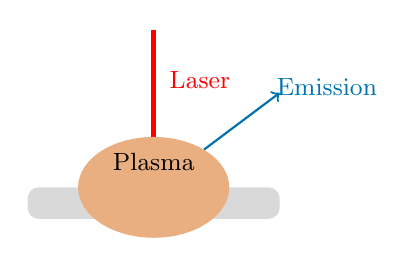
\begin{tikzpicture}[scale=0.8, every node/.style={font=\small}]
        \fill[gray!30, rounded corners] (0,0) rectangle (4,0.5);
        \node at (2,0.25) {Sample};
        \draw[->, red, ultra thick] (2,3) -- (2,0.6);
        \node[red, right] at (2.1,2.2) {Laser};
        \fill[cbOrange!50] (2,0.5) circle [x radius=1.2, y radius=0.8];
        \node at (2,0.9) {Plasma};
        \draw[->, cbBlue, thick] (2.8,1.1) -- (4,2);
        \node[cbBlue, right] at (3.8,2.1) {Emission};
      \end{tikzpicture}
    \end{column}
  \end{columns}

  \vspace{0.5em}
  \footnotesize NASA's ChemCam \& SuperCam instruments on Mars rovers use LIBS
\note{
  LIBS fires a laser at a target, creating a plasma whose emission lines
  reveal which elements are present and in what concentrations.
  It is used in geology, industry, and most famously aboard Mars rovers.
  The question is: can we go from spectrum to composition without calibration standards?
}
\end{frame}

% ----------------------------------------------------------
% SLIDE 3: What is CF-LIBS?
% ----------------------------------------------------------
\begin{frame}{Calibration-Free LIBS}
  \begin{block}{The idea: derive composition from plasma physics alone}
    No matrix-matched standards needed --- use first-principles equations.
  \end{block}

  \vspace{0.5em}
  \textbf{Three governing equations:}
  \begin{enumerate}
    \item \textbf{Boltzmann distribution} $\to$ excited-state populations from $T$
    \item \textbf{Saha equation} $\to$ ionization ratios from $T$ and $n_e$
    \item \textbf{Closure} $\to$ $\sum_i C_i = 1$ (all concentrations sum to unity)
  \end{enumerate}

  \vspace{0.5em}
  \alert{Problem:} Computationally intensive --- $10^4$--$10^5$ transitions,
  iterative self-consistency, Voigt profile evaluation for every line.
\note{
  CF-LIBS eliminates the need for reference standards by using the
  Boltzmann distribution, Saha equation, and a closure constraint.
  The catch is that solving this system is computationally expensive:
  many atomic transitions, iterative solvers, and Voigt profile convolutions.
  This is the bottleneck we address.
}
\end{frame}

% ----------------------------------------------------------
% SLIDE 4: Why GPU acceleration?
% ----------------------------------------------------------
\begin{frame}{Why GPU Acceleration?}
  \textbf{Real-time demands:}
  \begin{itemize}
    \item Laser repetition: 1--20 Hz, 10--100 spectra accumulated per analysis
    \item Need hundreds of spectra/second for online monitoring
    \item Manifold-based inference: $10^6$--$10^8$ synthetic spectra
  \end{itemize}

  \vspace{1em}
  \textbf{Prior GPU spectroscopy work:}
  \begin{description}
    \item[ExoJAX] (Kawahara+ 2022): $\sim$10,000 spectra/sec on V100 for exoplanet atmospheres
    \item[HELIOS-K] (Grimm+ 2021): CUDA C++ opacity calculator, high throughput
  \end{description}

  \vspace{0.5em}
  \alert{Gap:} No GPU-accelerated CF-LIBS implementation existed.\\
  Neither ExoJAX nor HELIOS-K handles the multi-element Saha--Boltzmann chain.
\note{
  Real-time LIBS at laser repetition rates and manifold generation
  over millions of spectra both demand much higher throughput than serial CPU code
  can provide. ExoJAX and HELIOS-K showed GPUs work for spectral
  computation, but neither handles the CF-LIBS pipeline.
  We fill that gap. Let me show you the architecture.
}
\end{frame}

% ----------------------------------------------------------
% SLIDE 5: Pipeline architecture
% ----------------------------------------------------------
\begin{frame}{Pipeline Architecture}
  \centering
  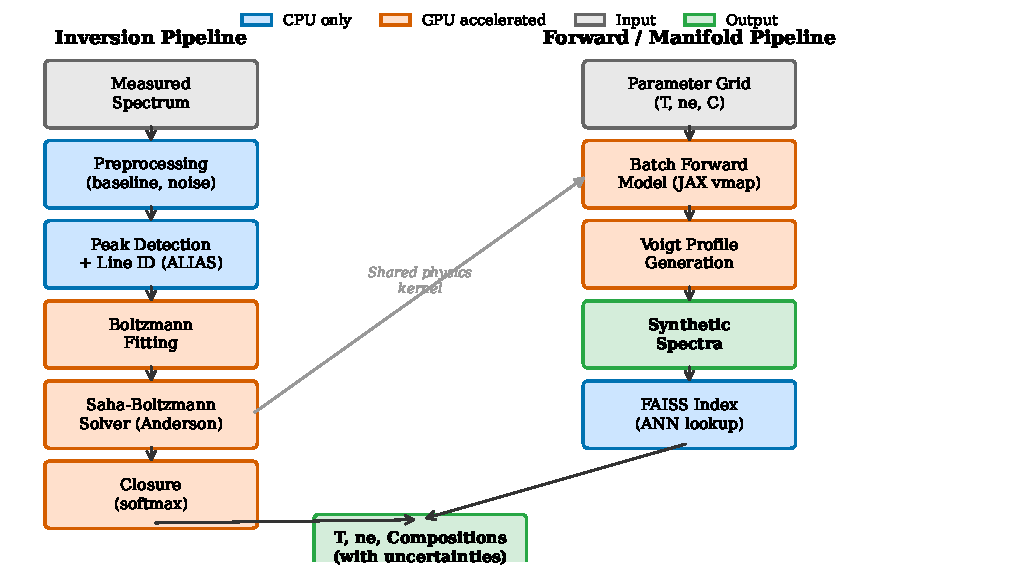
\includegraphics[width=0.92\textwidth]{../paper/figures/fig1_pipeline.pdf}

  \vspace{0.5em}
  {\small Five GPU-accelerated kernels (shaded) implemented in JAX:
  \texttt{jit} + \texttt{vmap} + \texttt{grad}}
\note{
  Here is the full pipeline. Five computational kernels, shown shaded,
  are GPU-accelerated via JAX. The key JAX features we exploit are
  just-in-time compilation, vectorization with vmap, and automatic
  differentiation with grad. Let me walk through each kernel.
}
\end{frame}

% ----------------------------------------------------------
% SLIDE 6: Why JAX?
% ----------------------------------------------------------
\begin{frame}{Why JAX?}
  \begin{columns}[T]
    \begin{column}{0.48\textwidth}
      \textbf{Three key capabilities:}
      \begin{enumerate}
        \item \texttt{jit} --- JIT compilation to GPU via XLA
        \item \texttt{vmap} --- automatic batch vectorization
        \item \texttt{grad} --- automatic differentiation
      \end{enumerate}

      \vspace{1em}
      \textbf{vs.\ hand-tuned CUDA:}
      \begin{itemize}
        \item Python-level development velocity
        \item Single code path for CPU + GPU
        \item Free Jacobians for optimization
      \end{itemize}
    \end{column}
    \begin{column}{0.48\textwidth}
      \begin{exampleblock}{Batch forward model}
        \texttt{batch\_spectrum =}\\
        \quad\texttt{jit(vmap(single\_spectrum))}\\[0.5em]
        One line transforms a single-spectrum\\
        function into a GPU-parallel batch.
      \end{exampleblock}
    \end{column}
  \end{columns}
\note{
  We chose JAX over hand-written CUDA for three reasons.
  First, jit compiles Python to optimized GPU kernels.
  Second, vmap gives us batch parallelism for free.
  Third, grad provides automatic differentiation, so we get exact
  Jacobians for joint optimization without manual derivation.
  Now let me describe the five kernels, starting with Voigt profiles.
}
\end{frame}

% ----------------------------------------------------------
% SLIDE 7: Kernel 1 — Voigt profiles
% ----------------------------------------------------------
\begin{frame}{Kernel 1: GPU Voigt Profile}
  \textbf{Challenge:} Evaluate Faddeeva function $w(z)$ on GPU
  \begin{itemize}
    \item Standard Humlicek W4 algorithm uses conditional branches\\
          $\to$ warp divergence, incompatible with \texttt{jit}/\texttt{grad}
  \end{itemize}

  \vspace{0.5em}
  \textbf{Solution:} Weideman $N\!=\!36$ rational approximation
  \begin{equation*}
    w(z) \approx \frac{1}{\sqrt{\pi}} \frac{L}{L - iz}
      + \frac{2}{(L - iz)^2} \sum_{n=0}^{35} c_n Z^n
  \end{equation*}

  \begin{itemize}
    \item \alert{Branch-free} --- no conditionals, pure arithmetic
    \item 236 FLOPs per evaluation
    \item Max relative error $< 10^{-13}$ in float64
    \item Full $(N_\text{wl} \times N_\text{lines})$ matrix in a single XLA kernel
  \end{itemize}
\note{
  The Voigt profile is a convolution of Gaussian and Lorentzian shapes.
  Evaluating it requires the Faddeeva function.
  The standard Humlicek algorithm branches on input values, causing
  GPU warp divergence. We use the Weideman N=36 rational approximation,
  which is entirely branch-free: 236 floating-point operations,
  no conditionals. The entire wavelength-by-lines matrix is computed
  as a single fused GPU kernel. Let me show you the speedup.
}
\end{frame}

% ----------------------------------------------------------
% SLIDE 8: Voigt results
% ----------------------------------------------------------
\begin{frame}{Voigt Profile: 76$\times$ Speedup}
  \begin{columns}[T]
    \begin{column}{0.52\textwidth}
      \centering
      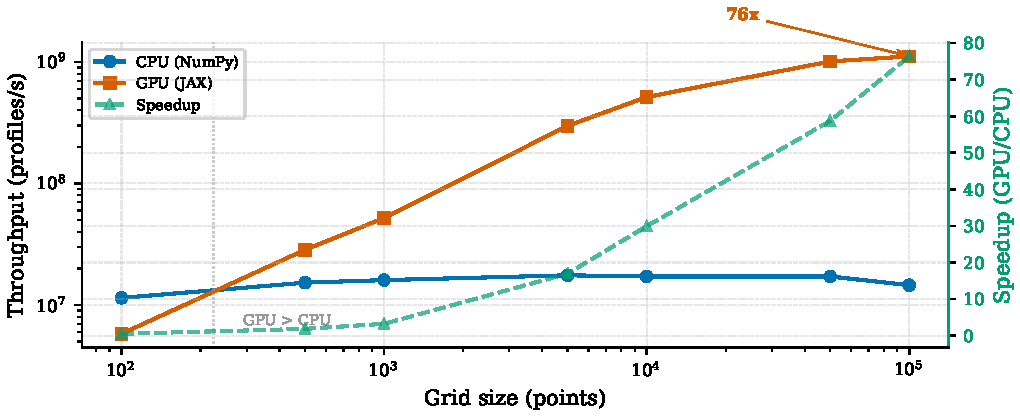
\includegraphics[width=\textwidth]{../paper/figures/fig2_voigt.pdf}
    \end{column}
    \begin{column}{0.45\textwidth}
      \textbf{Key numbers:}
      \begin{itemize}
        \item \alert{76.4$\times$} speedup at $10^5$ grid points
        \item GPU: $1.1 \times 10^9$ Faddeeva evals/sec
        \item CPU: $1.5 \times 10^7$ evals/sec
        \item Crossover at $\sim$500 grid points
      \end{itemize}

      \vspace{0.5em}
      \textbf{Accuracy:}\\
      Max relative error: $5.07 \times 10^{-14}$\\
      {\small(vs.\ SciPy Poppe--Wijers reference)}
    \end{column}
  \end{columns}
\note{
  At 100,000 wavelength grid points, the GPU evaluates Faddeeva functions
  76 times faster than CPU, processing over a billion evaluations per second.
  The numerical error is 5 times 10 to the minus 14 --- essentially
  machine precision. The crossover where GPU beats CPU is only 500 grid points,
  well below any real LIBS spectrum. Next: Boltzmann fitting.
}
\end{frame}

% ----------------------------------------------------------
% SLIDE 9: Kernel 2 — Boltzmann fitting
% ----------------------------------------------------------
\begin{frame}{Kernel 2: Vectorized Boltzmann Fitting}
  \textbf{Boltzmann plot method:}
  \begin{equation*}
    \ln\!\left(\frac{I \lambda}{g_k A_{ki}}\right) = -\frac{E_k}{k_B T} + \text{const}
  \end{equation*}

  \vspace{0.3em}
  \textbf{Challenge:} Different elements have different numbers of lines (ragged arrays)

  \vspace{0.3em}
  \textbf{Solution:} Closed-form WLS + pad-and-mask batching
  \begin{itemize}
    \item Five dot-product accumulators $\to$ slope and intercept
    \item Pad all elements to $N_\text{max}$ lines, mask out padding
    \item Element dimension = batch axis $\to$ parallel GPU execution
    \item Only $10 N_\text{max} + 7$ FLOPs per element
  \end{itemize}
\note{
  The Boltzmann plot extracts temperature from line intensities.
  The challenge is that each element has a different number of
  emission lines, creating ragged arrays.
  We solved this with a pad-and-mask strategy: all elements padded
  to a common length, with zero-weight masks on padding entries.
  The closed-form weighted least squares needs only five dot products.
}
\end{frame}

% ----------------------------------------------------------
% SLIDE 10: Boltzmann results
% ----------------------------------------------------------
\begin{frame}{Boltzmann Fitting: 8.8$\times$ Speedup}
  \begin{columns}[T]
    \begin{column}{0.52\textwidth}
      \centering
      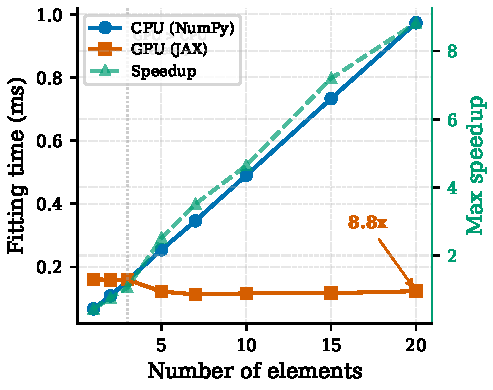
\includegraphics[width=\textwidth]{../paper/figures/fig3_boltzmann.pdf}
    \end{column}
    \begin{column}{0.45\textwidth}
      \textbf{Key numbers:}
      \begin{itemize}
        \item \alert{8.8$\times$} speedup at 20 elements
        \item GPU time nearly constant: $\sim$0.12 ms regardless of $D$
        \item CPU time scales linearly with $D$
        \item Break-even at $\sim$3 elements
      \end{itemize}

      \vspace{0.5em}
      \textbf{Accuracy:}\\
      Slope relative error: $5.65 \times 10^{-14}$
    \end{column}
  \end{columns}
\note{
  At 20 elements, the GPU is 8.8 times faster.
  The important feature is that GPU time is essentially constant
  regardless of how many elements you have --- it is all
  executed in parallel. CPU time grows linearly.
  The slope error is at machine precision.
  Next: the iterative Saha-Boltzmann solver.
}
\end{frame}

% ----------------------------------------------------------
% SLIDE 11: Kernel 3 — Anderson acceleration
% ----------------------------------------------------------
\begin{frame}{Kernel 3: Anderson-Accelerated Saha Solver}
  \textbf{Fixed-point problem:} $n_e = g(n_e)$ via charge neutrality

  \vspace{0.5em}
  \textbf{Simple Picard iteration:} $n_e^{(k+1)} = g(n_e^{(k)})$
  \begin{itemize}
    \item Converges, but rate depends on $|g'(n_e^*)|$
  \end{itemize}

  \vspace{0.3em}
  \textbf{Anderson acceleration:} store $m$ previous iterates, solve least-squares
  \begin{equation*}
    n_e^{(k+1)} = g(n_e^{(k)}) - (\Delta G_k + \Delta R_k)\, \bm{\gamma}_k^*
  \end{equation*}

  \begin{itemize}
    \item Optimal depth $m = 1$ at tolerance $10^{-6}$
    \item Implemented via \texttt{lax.scan} --- static computation graph
    \item Reduces to Picard when $m = 0$ (zero-cost fallback)
  \end{itemize}
\note{
  The Saha-Boltzmann loop requires iterating electron density
  to self-consistency. Anderson acceleration stores previous iterates
  and finds an optimal linear combination to accelerate convergence.
  We implement it with JAX's lax.scan for a static computation graph.
  At m=0 it falls back to plain Picard iteration at no extra cost.
}
\end{frame}

% ----------------------------------------------------------
% SLIDE 12: Anderson results
% ----------------------------------------------------------
\begin{frame}{Anderson Convergence: 1.6$\times$ Iteration Reduction}
  \begin{columns}[T]
    \begin{column}{0.52\textwidth}
      \centering
      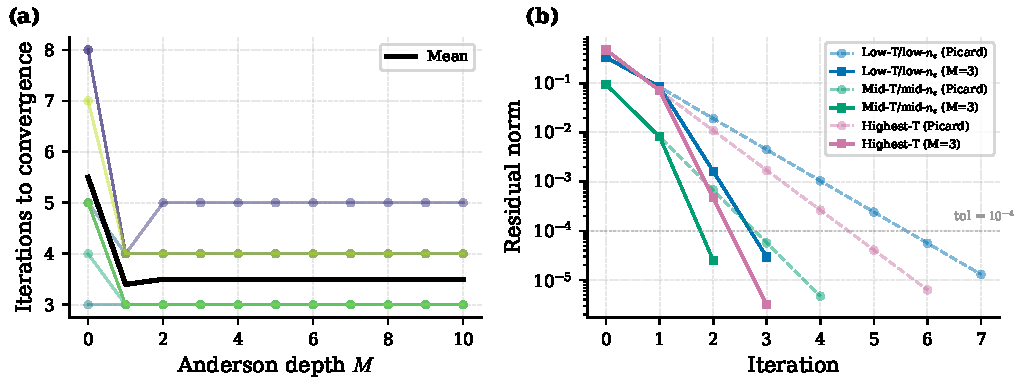
\includegraphics[width=\textwidth]{../paper/figures/fig4_anderson.pdf}
    \end{column}
    \begin{column}{0.45\textwidth}
      \textbf{Key numbers:}
      \begin{itemize}
        \item \alert{1.6$\times$} avg.\ iteration reduction
        \item Hardest case: 7 $\to$ 4 iterations
        \item Tighter tolerance: $m\!=\!5$ gives $2.9\times$
      \end{itemize}

      \vspace{0.5em}
      \textbf{Honest assessment:}\\
      Modest for typical LIBS plasmas\\
      (Picard contraction $|g'| \sim 0.3$--$0.7$)\\[0.3em]
      Most valuable for:
      \begin{itemize}
        \item High-$T$ ($>$ 2 eV) plasmas
        \item Tight tolerances ($< 10^{-10}$)
      \end{itemize}
    \end{column}
  \end{columns}
\note{
  Anderson acceleration gives a 1.6x average iteration reduction.
  This is honest: for typical LIBS conditions, Picard already converges
  in 3 to 8 steps, so the improvement is modest.
  The real value is a convergence guarantee for harder conditions ---
  high temperature, multiply ionized plasmas --- and at tighter
  tolerances where depth m=5 gives a 2.9x reduction.
}
\end{frame}

% ----------------------------------------------------------
% SLIDE 13: Kernel 4 — Softmax closure
% ----------------------------------------------------------
\begin{frame}{Kernel 4: Softmax Compositional Closure}
  \textbf{Constraint:} $\sum_{i=1}^D C_i = 1$, \quad $C_i > 0$

  \vspace{0.5em}
  \textbf{Traditional approach:} Normalize after each iteration\\
  $\to$ breaks gradient flow, numerically fragile at simplex boundary

  \vspace{0.5em}
  \textbf{Softmax reparameterization:}
  \begin{equation*}
    C_i = \frac{\exp(\theta_i)}{\sum_{j} \exp(\theta_j)}
    \qquad\text{(log-sum-exp trick for stability)}
  \end{equation*}

  \begin{itemize}
    \item Constraint satisfied \alert{exactly by construction}
    \item Strict positivity for all finite $\bm{\theta}$
    \item Exact Jacobian: $J_{ij} = C_i(\delta_{ij} - C_j)$
    \item Enables gradient-based joint optimization of $T$, $n_e$, $\bm{C}$
  \end{itemize}

  \vspace{0.3em}
  Accuracy: max deviation $4.44 \times 10^{-16}$ (machine epsilon)
\note{
  CF-LIBS compositions must sum to one and be positive.
  Traditional normalization breaks gradient flow.
  The softmax reparameterization maps unconstrained parameters
  to the probability simplex exactly by construction.
  The analytic Jacobian enables joint gradient-based optimization
  of temperature, electron density, and all concentrations simultaneously.
  Accuracy is at machine epsilon.
}
\end{frame}

% ----------------------------------------------------------
% SLIDE 14: Kernel 5 — Batch forward model
% ----------------------------------------------------------
\begin{frame}{Kernel 5: Batch Forward Model}
  \textbf{Forward model:} $(T, n_e, \bm{C}) \to$ synthetic spectrum $S(\lambda)$

  \vspace{0.3em}
  Four stages: Saha ionization $\to$ Boltzmann populations $\to$ line emissivity $\to$ Voigt broadening

  \vspace{0.5em}
  \textbf{Batch via \texttt{vmap}:}
  \begin{equation*}
    \texttt{batch\_spectrum} = \texttt{jit}(\texttt{vmap}(\texttt{single\_spectrum}))
  \end{equation*}

  \begin{itemize}
    \item Wavelength grid and atomic data \alert{shared} (broadcast)
    \item $(T, n_e, \bm{C})$ \alert{mapped} over batch dimension
    \item Profile matrix: $(B \times N_\text{wl} \times N_\text{lines})$ --- dominant memory cost
    \item \texttt{vmap} is a semantic transform: \alert{bit-identical} to sequential
  \end{itemize}
\note{
  The batch forward model composes all four kernels into a single
  vectorized pipeline. JAX's vmap maps over the batch dimension
  while sharing the wavelength grid and atomic database.
  Because vmap is a purely semantic transformation, it produces
  bit-identical results to sequential evaluation --- a strong
  correctness guarantee. Let me show you the throughput numbers.
}
\end{frame}

% ----------------------------------------------------------
% SLIDE 15: Batch forward results
% ----------------------------------------------------------
\begin{frame}{Batch Throughput: 10,708 Spectra/sec}
  \begin{columns}[T]
    \begin{column}{0.52\textwidth}
      \centering
      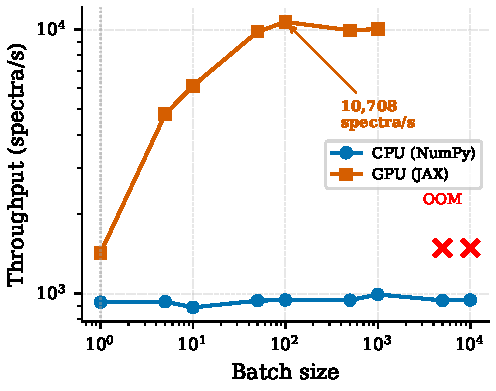
\includegraphics[width=\textwidth]{../paper/figures/fig6_batch.pdf}
    \end{column}
    \begin{column}{0.45\textwidth}
      \textbf{Key numbers:}
      \begin{itemize}
        \item \alert{10,708} spectra/sec peak ($B\!=\!100$)
        \item GPU saturates at $B \geq 50$
        \item CPU: $\sim$940 spectra/sec (constant)
        \item 11.3$\times$ speedup at peak
      \end{itemize}

      \vspace{0.5em}
      \textbf{Memory limit:}\\
      OOM at $B \geq 5000$ on 32 GB V100S\\
      Chunked execution recovers full throughput
    \end{column}
  \end{columns}
\note{
  Peak throughput is 10,708 spectra per second at batch size 100.
  This is comparable to ExoJAX's 10,000 spectra per second
  on the same GPU, even though our pipeline is more complex.
  GPU memory limits the maximum batch size to about 5000 on this hardware,
  but chunked execution handles larger workloads transparently.
}
\end{frame}

% ----------------------------------------------------------
% SLIDE 16: End-to-end pipeline
% ----------------------------------------------------------
\begin{frame}{End-to-End Pipeline: 13.6$\times$ Speedup}
  \begin{columns}[T]
    \begin{column}{0.52\textwidth}
      \centering
      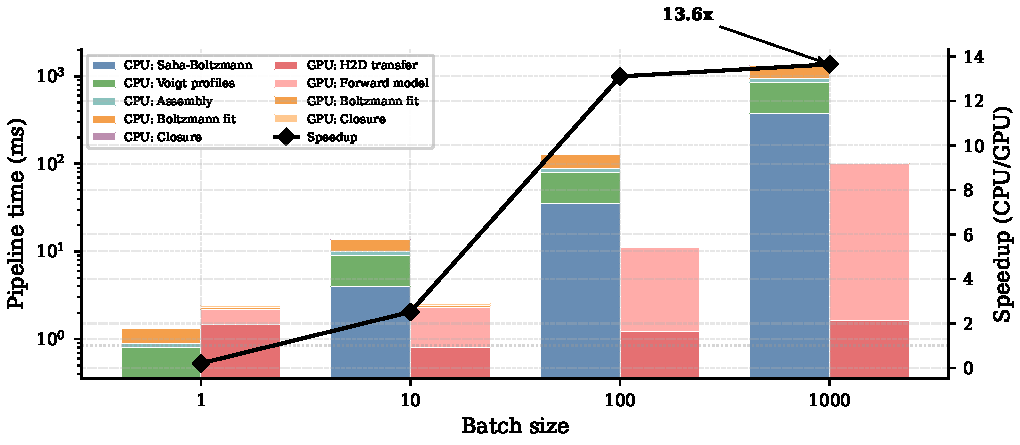
\includegraphics[width=\textwidth]{../paper/figures/fig7_e2e.pdf}
    \end{column}
    \begin{column}{0.45\textwidth}
      \textbf{Key numbers:}
      \begin{itemize}
        \item \alert{13.6$\times$} at batch size 1000
        \item Crossover at $B \geq 10$
        \item At $B\!=\!1$: GPU is $4.8\times$ \emph{slower}
      \end{itemize}

      \vspace{0.5em}
      \textbf{CPU bottleneck breakdown} ($B\!=\!1000$):
      \begin{itemize}
        \item Voigt profiles: 34.7\%
        \item Saha--Boltzmann: 27.8\%
        \item Boltzmann fit: 27.8\%
        \item Closure + prep: $<$1\%
      \end{itemize}
    \end{column}
  \end{columns}
\note{
  The end-to-end pipeline achieves 13.6x speedup at batch 1000.
  The crossover is at batch size 10 --- above that, GPU wins.
  At batch 1, GPU is slower due to kernel launch overhead.
  On CPU, Voigt profiles consume 35 percent of the time, followed
  by Saha-Boltzmann and Boltzmann fitting at 28 percent each.
  The GPU parallelizes all three bottlenecks simultaneously.
}
\end{frame}

% ----------------------------------------------------------
% SLIDE 17: Accuracy summary
% ----------------------------------------------------------
\begin{frame}{Numerical Accuracy: Zero Precision Loss}
  \centering
  \begin{tabular}{lccc}
    \toprule
    \textbf{Kernel} & \textbf{Threshold} & \textbf{Achieved} & \textbf{$N_\text{tests}$} \\
    \midrule
    Voigt profile   & $10^{-6}$  & $6.81 \times 10^{-8}$  & 410  \\
    Boltzmann fit   & $10^{-10}$ & $5.65 \times 10^{-14}$ & 1000 \\
    Anderson solver & $10^{-12}$ & $4.05 \times 10^{-13}$ & 60   \\
    Softmax closure & $10^{-15}$ & $4.44 \times 10^{-16}$ & 1009 \\
    Batch forward   & $10^{-12}$ & $0.0$ (bit-identical)   & 100  \\
    \bottomrule
  \end{tabular}

  \vspace{1em}
  All kernels beat their thresholds by \alert{orders of magnitude}.\\
  Float64 arithmetic throughout --- no mixed-precision compromises.
\note{
  This table summarizes accuracy across all five kernels.
  Every kernel beats its threshold by orders of magnitude.
  The batch forward model is bit-identical to sequential computation.
  We use float64 throughout --- no mixed-precision shortcuts.
  All numbers verified against SciPy and CPU reference implementations
  over hundreds to thousands of test cases.
}
\end{frame}

% ----------------------------------------------------------
% SLIDE 18: Real-data validation — Aalto
% ----------------------------------------------------------
\begin{frame}{Real-Data Validation}
  \begin{columns}[T]
    \begin{column}{0.48\textwidth}
      \textbf{Aalto University LIBS Library}
      \begin{itemize}
        \item 74 spectra (13 pure elements, 61 minerals)
        \item \alert{100\% GPU--CPU parity} across all kernels
        \item Per-kernel max errors:
        \begin{itemize}
          \item Boltzmann: $1.0 \times 10^{-14}$
          \item Voigt: $4.5 \times 10^{-16}$
          \item Softmax: $2.0 \times 10^{-16}$
          \item Charge balance: $2.5 \times 10^{-9}$
        \end{itemize}
      \end{itemize}
    \end{column}
    \begin{column}{0.48\textwidth}
      \textbf{ChemCam CCCT Targets}
      \begin{itemize}
        \item 6 calibration targets (CCCT-1 to CCCT-5, CCCT-9)
        \item Certified compositions (Fabre+ 2011)
        \item \alert{100\% pass rate} on all kernel parity tests
        \item 19/19 major elements correctly detected
      \end{itemize}
    \end{column}
  \end{columns}

  \vspace{0.5em}
  \centering
  GPU--CPU parity confirmed on \alert{real experimental data}, not just synthetic tests.
\note{
  We validated on real data from two independent sources.
  The Aalto library gives us 74 spectra of pure elements and minerals ---
  100 percent GPU-CPU parity. The ChemCam calibration targets
  with certified compositions also show 100 percent pass rate.
  This confirms the GPU implementation is correct on real-world data,
  not just synthetic test cases.
}
\end{frame}

% ----------------------------------------------------------
% SLIDE 19: Comparison with prior work
% ----------------------------------------------------------
\begin{frame}{Context: GPU Spectroscopy Landscape}
  \centering
  \begin{tabular}{lccl}
    \toprule
    \textbf{Code} & \textbf{Throughput} & \textbf{Language} & \textbf{Application} \\
    \midrule
    ExoJAX       & $\sim$10,000 spec/s & JAX/Python    & Exoplanet atmospheres \\
    HELIOS-K     & Higher              & CUDA C++      & Exoplanet opacity \\
    \alert{This work} & \alert{10,708 spec/s}  & \alert{JAX/Python} & \alert{CF-LIBS} \\
    \bottomrule
  \end{tabular}

  \vspace{1em}
  \begin{itemize}
    \item Comparable throughput to ExoJAX despite \emph{more complex} physics\\
          (multi-element Saha--Boltzmann chain vs.\ single-species opacity sum)
    \item JAX advantage over CUDA C++: automatic differentiation for free\\
          $\to$ gradient-based joint optimization, Bayesian inference via HMC
    \item Modest performance cost pays for enormous development flexibility
  \end{itemize}
\note{
  Our throughput matches ExoJAX even though our pipeline is more complex ---
  we have a full multi-element Saha-Boltzmann chain, not just an opacity sum.
  Compared to HELIOS-K's hand-tuned CUDA, JAX trades some raw speed
  for automatic differentiation --- which gives us gradient-based optimization
  and Bayesian inference without manually deriving Jacobians.
  That is a major practical advantage for the CF-LIBS inversion problem.
}
\end{frame}

% ----------------------------------------------------------
% SLIDE 20: Operating regimes
% ----------------------------------------------------------
\begin{frame}{When to Use GPU vs.\ CPU}
  \centering
  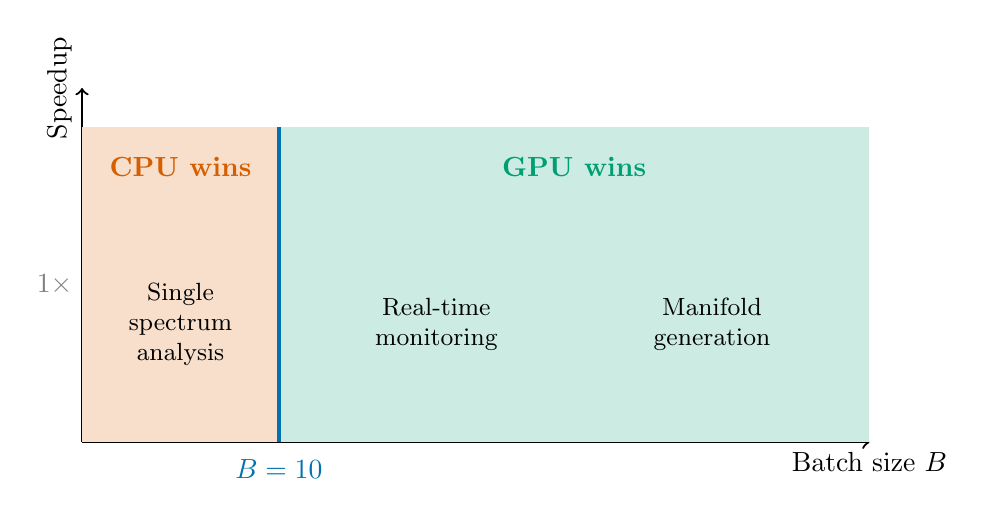
\begin{tikzpicture}[scale=1.0]
    % Axis
    \draw[->, thick] (0,0) -- (10,0) node[below] {Batch size $B$};
    \draw[->, thick] (0,0) -- (0,4.5) node[left, rotate=90, anchor=south] {Speedup};
    % Crossover line
    \draw[dashed, gray] (0,2) -- (10,2);
    \node[left, gray] at (0,2) {1$\times$};
    % Regions
    \fill[cbOrange!20] (0,0) rectangle (2.5,4);
    \fill[cbGreen!20] (2.5,0) rectangle (10,4);
    \node[cbOrange, font=\bfseries] at (1.25,3.5) {CPU wins};
    \node[cbGreen, font=\bfseries] at (6.25,3.5) {GPU wins};
    % Crossover point
    \draw[cbBlue, ultra thick] (2.5,0) -- (2.5,4);
    \node[cbBlue, below, font=\bfseries] at (2.5,-0.1) {$B = 10$};
    % Annotations
    \node[align=center, font=\small] at (1.25,1.5) {Single\\spectrum\\analysis};
    \node[align=center, font=\small] at (4.5,1.5) {Real-time\\monitoring};
    \node[align=center, font=\small] at (8,1.5) {Manifold\\generation};
  \end{tikzpicture}

  \vspace{0.5em}
  \begin{itemize}
    \item $B < 10$: Use CPU (kernel launch overhead dominates)
    \item $B = 10$--1000: GPU provides 2.5$\times$--13.6$\times$ speedup
    \item $B > 5000$: Chunk into sub-batches to fit GPU memory
  \end{itemize}
\note{
  This diagram summarizes when to use GPU versus CPU.
  Below batch size 10, stick with CPU.
  Between 10 and 1000, GPU gives 2.5 to 13.6 times speedup ---
  this is the sweet spot for real-time monitoring.
  Above 5000, chunk the computation to fit GPU memory.
  The take-home: GPU acceleration is practical for any batch workload.
}
\end{frame}

% ----------------------------------------------------------
% SLIDE 21: Limitations
% ----------------------------------------------------------
\begin{frame}{Limitations and Caveats}
  \begin{itemize}
    \item \textbf{Hardware-specific benchmarks:} All numbers from Tesla V100S\\
          Consumer GPUs with $1/32$ float64 rate would see lower speedups
    \item \textbf{LTE assumption:} Single-zone, optically thin, LTE only\\
          Non-LTE and self-absorption not yet GPU-accelerated
    \item \textbf{JIT compilation overhead:} 30--120 s first call\\
          Amortized over subsequent calls ($<$0.01\% for manifolds)
    \item \textbf{Float64 required:} Weideman coefficients span 14 orders of magnitude\\
          Float32 would double throughput but introduce $\sim$0.1--1\% errors
    \item \textbf{GPU FAISS:} Not benchmarked (null results on test system)
  \end{itemize}
\note{
  Some important caveats. These benchmarks are on a V100S ---
  consumer GPUs would see lower speedups due to poor float64 support.
  We assume LTE, single zone, optically thin plasmas.
  JIT compilation takes 30 to 120 seconds on first call, but this
  is negligible for batch workloads. We require float64 for accuracy.
  GPU FAISS remains untested and is future work.
}
\end{frame}

% ----------------------------------------------------------
% SLIDE 22: Future directions
% ----------------------------------------------------------
\begin{frame}{Future Directions}
  \begin{enumerate}
    \item \textbf{Multi-GPU scaling:} \texttt{pmap} for manifold generation at $10^6$+ spectra
    \item \textbf{Non-LTE extensions:} Collisional-radiative models on GPU
    \item \textbf{Mixed-precision:} Float32 profiles + float64 coefficients\\
          $\to$ $\sim$2$\times$ additional throughput where $\sim$0.1\% accuracy suffices
    \item \textbf{GPU FAISS:} Complete the GPU inference chain
    \item \textbf{Edge deployment:} Jetson / Apple Neural Engine for field-portable LIBS
  \end{enumerate}

  \vspace{1em}
  \begin{block}{Open source}
    Code, benchmarks, and validation data publicly available.
  \end{block}
\note{
  Several directions are ongoing. Multi-GPU scaling for large manifolds.
  Non-LTE extensions to broaden applicability.
  Mixed precision for applications where 0.1 percent accuracy is fine.
  GPU FAISS to complete the inference chain. And edge deployment
  on embedded GPUs for field-portable instruments.
  All code is open source.
}
\end{frame}

% ----------------------------------------------------------
% SLIDE 23: Conclusions
% ----------------------------------------------------------
\begin{frame}{Conclusions}
  \begin{enumerate}
    \item First GPU-accelerated CF-LIBS implementation
    \item Five kernels optimized: Voigt (\alert{76$\times$}), Boltzmann (\alert{8.8$\times$}),
          Anderson (\alert{1.6$\times$} iterations), Softmax (exact Jacobian),
          Batch forward (\alert{10,708} spec/s)
    \item End-to-end: \alert{13.6$\times$} at $B\!=\!1000$, crossover at $B \geq 10$
    \item \alert{Zero accuracy loss} --- all kernels pass precision thresholds
    \item Validated on 74 Aalto spectra + 6 ChemCam targets: 100\% parity
    \item JAX framework: GPU + autodiff + Python in a single codebase
  \end{enumerate}

  \vspace{0.5em}
  \centering
  \textbf{GPU-accelerated CF-LIBS is ready for real-time deployment.}
\note{
  To summarize: this is the first GPU-accelerated CF-LIBS implementation.
  Five kernels, up to 76x individual speedup, 13.6x end-to-end,
  with zero accuracy loss validated on real experimental data.
  The JAX framework gives us GPU acceleration, automatic differentiation,
  and Python development velocity in a single codebase.
  GPU-accelerated CF-LIBS is ready for real-time deployment.
}
\end{frame}

% ----------------------------------------------------------
% SLIDE 24: Thank you
% ----------------------------------------------------------
\begin{frame}[standout]
  Thank you

  \vspace{1em}
  {\large Questions?}

  \vspace{1.5em}
  {\normalsize Code: \texttt{github.com/[repository]}}
\note{
  Thank you for your attention. I am happy to take questions.
  The code is publicly available on GitHub.
}
\end{frame}

% ============================================================
% BACKUP SLIDES
% ============================================================
\appendix

\begin{frame}{Backup Slides}
  \centering
  {\Large Additional detail for Q\&A}
\note{
  The following slides provide additional detail for anticipated questions.
}
\end{frame}

% ----------------------------------------------------------
% BACKUP 1: Full accuracy table
% ----------------------------------------------------------
\begin{frame}{Backup: Full Accuracy Table}
  \centering
  \begin{tabular}{lcccc}
    \toprule
    \textbf{Kernel} & \textbf{Threshold} & \textbf{Achieved} & \textbf{$N_\text{tests}$} & \textbf{Unit} \\
    \midrule
    Voigt profile   & $10^{-6}$  & $6.81 \times 10^{-8}$  & 410  & rel.\ error \\
    Boltzmann fit   & $10^{-10}$ & $5.65 \times 10^{-14}$ & 1000 & rel.\ error (slope) \\
    Anderson solver & $10^{-12}$ & $4.05 \times 10^{-13}$ & 60   & abs.\ residual \\
    Softmax closure & $10^{-15}$ & $4.44 \times 10^{-16}$ & 1009 & abs.\ deviation \\
    Batch forward   & $10^{-12}$ & $0.0$ (bit-identical)   & 100  & rel.\ error \\
    \bottomrule
  \end{tabular}

  \vspace{1em}
  \textbf{References:}
  \begin{itemize}
    \item Voigt: vs.\ SciPy \texttt{wofz} (Poppe--Wijers Algorithm 680)
    \item Boltzmann: vs.\ NumPy \texttt{lstsq} reference
    \item Anderson: final residual $|n_e^{(k+1)} - g(n_e^{(k)})|$
    \item Softmax: $|\sum C_i - 1|$
    \item Batch: vs.\ sequential \texttt{for}-loop computation
  \end{itemize}
\note{
  This slide gives the full accuracy table with units and reference
  implementations. Every kernel is compared against an independent
  CPU reference. The batch forward model achieves exact bit-identity.
}
\end{frame}

% ----------------------------------------------------------
% BACKUP 2: Anderson convergence detail
% ----------------------------------------------------------
\begin{frame}{Backup: Anderson Convergence Detail}
  \centering
  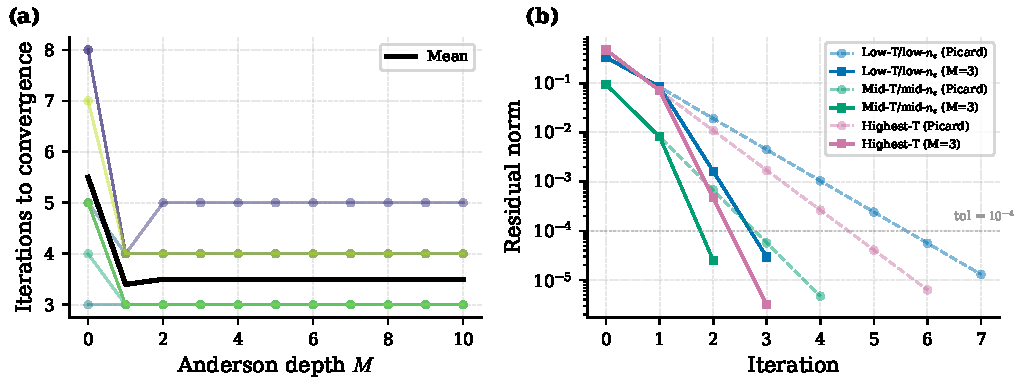
\includegraphics[width=0.7\textwidth]{../paper/figures/fig4_anderson.pdf}

  \vspace{0.5em}
  \begin{itemize}
    \item 10 test conditions: $T = 0.6$--$1.5$ eV, $n_e = 10^{15}$--$10^{17}$ cm$^{-3}$
    \item $m = 1$ optimal at tol $= 10^{-6}$; $m = 5$ optimal at tighter tolerances
    \item $m \geq 2$ adds least-squares overhead without reducing iterations at $10^{-6}$
    \item Convergence proved by Toth \& Kelley (2015): r-linear with improved rate
  \end{itemize}
\note{
  Anderson acceleration was tested across 10 plasma conditions.
  At standard tolerance, depth m=1 is optimal because the problem
  is already well-conditioned. For tighter tolerances or harder
  conditions, deeper history helps significantly.
}
\end{frame}

% ----------------------------------------------------------
% BACKUP 3: Batch forward OOM analysis
% ----------------------------------------------------------
\begin{frame}{Backup: Memory Scaling and OOM Analysis}
  \textbf{Dominant memory consumer:} Profile matrix $(B \times N_\text{wl} \times N_\text{lines})$

  \begin{equation*}
    B_\text{max} = \left\lfloor \frac{M_\text{GPU} - M_\text{overhead}}{N_\text{wl} \times N_\text{lines} \times 8\;\text{bytes}} \right\rfloor
  \end{equation*}

  \vspace{0.5em}
  \centering
  \begin{tabular}{rcc}
    \toprule
    \textbf{Batch size} & \textbf{Est.\ memory} & \textbf{Status} \\
    \midrule
    100   & $\sim$0.16 GB & OK \\
    1000  & $\sim$1.6 GB  & OK \\
    5000  & $\sim$8.2 GB  & OOM on 32 GB V100S \\
    10000 & $\sim$91.6 GB & OOM (E2E pipeline) \\
    \bottomrule
  \end{tabular}

  \vspace{0.5em}
  \textbf{Mitigation:} Chunked execution --- process $B_\text{max}$ at a time, concatenate.\\
  Full throughput recovered with minimal inter-chunk overhead.
\note{
  The profile matrix dominates GPU memory. This table shows the estimated
  memory for different batch sizes. At 5000, the isolated forward model
  exceeds memory; the full pipeline hits OOM earlier because of
  additional intermediate arrays. Chunking is the standard solution.
}
\end{frame}

% ----------------------------------------------------------
% BACKUP 4: FAISS CPU-only results
% ----------------------------------------------------------
\begin{frame}{Backup: FAISS Manifold Query (CPU Only)}
  \centering
  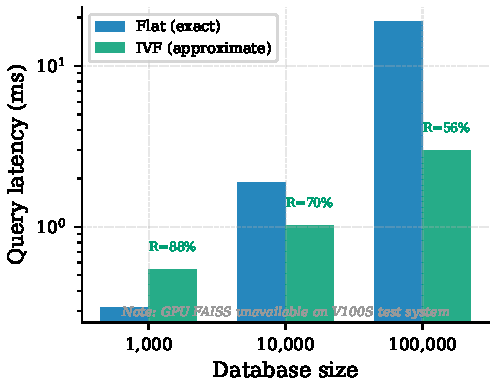
\includegraphics[width=0.65\textwidth]{../paper/figures/fig5_faiss.pdf}

  \vspace{0.5em}
  \begin{itemize}
    \item FAISS nearest-neighbor search for manifold-based inference
    \item GPU FAISS benchmarks returned null on V100S test system
    \item CPU-only latency shown for reference
    \item GPU FAISS expected to provide significant speedup at $>10^6$ manifold entries
    \item Completing the GPU inference chain is an active future direction
  \end{itemize}
\note{
  FAISS provides nearest-neighbor search in the precomputed spectral manifold.
  We could not get GPU FAISS results on our test system --- only CPU
  timings are available. GPU FAISS acceleration is expected to help
  at large manifold sizes and remains future work.
}
\end{frame}

% ----------------------------------------------------------
% BACKUP 5: Derivation highlights
% ----------------------------------------------------------
\begin{frame}{Backup: Key Mathematical Details}
  \textbf{Voigt --- Weideman $N\!=\!36$:}
  \begin{itemize}
    \item M\"obius transform: $Z = (L + iz)/(L - iz)$, $L \approx 5.0454$
    \item Degree-35 polynomial in $Z$, 236 FLOPs
    \item Branch-free $\to$ no warp divergence, compatible with \texttt{grad}
  \end{itemize}

  \vspace{0.5em}
  \textbf{Boltzmann --- Closed-form WLS:}
  \begin{equation*}
    b = \frac{S_w S_{wxy} - S_{wx} S_{wy}}{S_w S_{wxx} - S_{wx}^2}, \qquad
    T = \frac{-1}{b \cdot k_B}
  \end{equation*}

  \vspace{0.3em}
  \textbf{Softmax Jacobian:}
  \begin{equation*}
    J_{ij} = C_i(\delta_{ij} - C_j) \qquad \text{(rank $D\!-\!1$, $\kappa = 1$ at uniform)}
  \end{equation*}
\note{
  This slide collects the key mathematical details for reference.
  The Weideman approximation uses a Mobius transform to map the
  upper half-plane to the unit disk, then evaluates a polynomial.
  The Boltzmann WLS solution is fully analytic.
  The softmax Jacobian has condition number 1 at uniform composition.
}
\end{frame}

\end{document}
